%% PMSC Architecture Diagram - TikZ/LaTeX Implementation
%% Author: Ege Berk Türk
%% Date: May 23, 2026
%% Usage: Compile with pdflatex or include in main.tex

\documentclass[border=10pt]{standalone}
\usepackage{tikz}
\usetikzlibrary{shapes.geometric, arrows.meta, positioning, fit, backgrounds, calc}

\tikzset{
  box/.style={rectangle, draw, fill=blue!20, thick, minimum height=1cm, minimum width=3cm, text centered},
  databox/.style={rectangle, draw, fill=green!20, thick, minimum height=0.8cm, minimum width=2.5cm, text centered},
  process/.style={rectangle, draw, fill=orange!30, thick, minimum height=1cm, minimum width=3.5cm, text centered, rounded corners=5pt},
  arrow/.style={-Stealth, thick},
  label/.style={font=\small\ttfamily},
}

\begin{document}
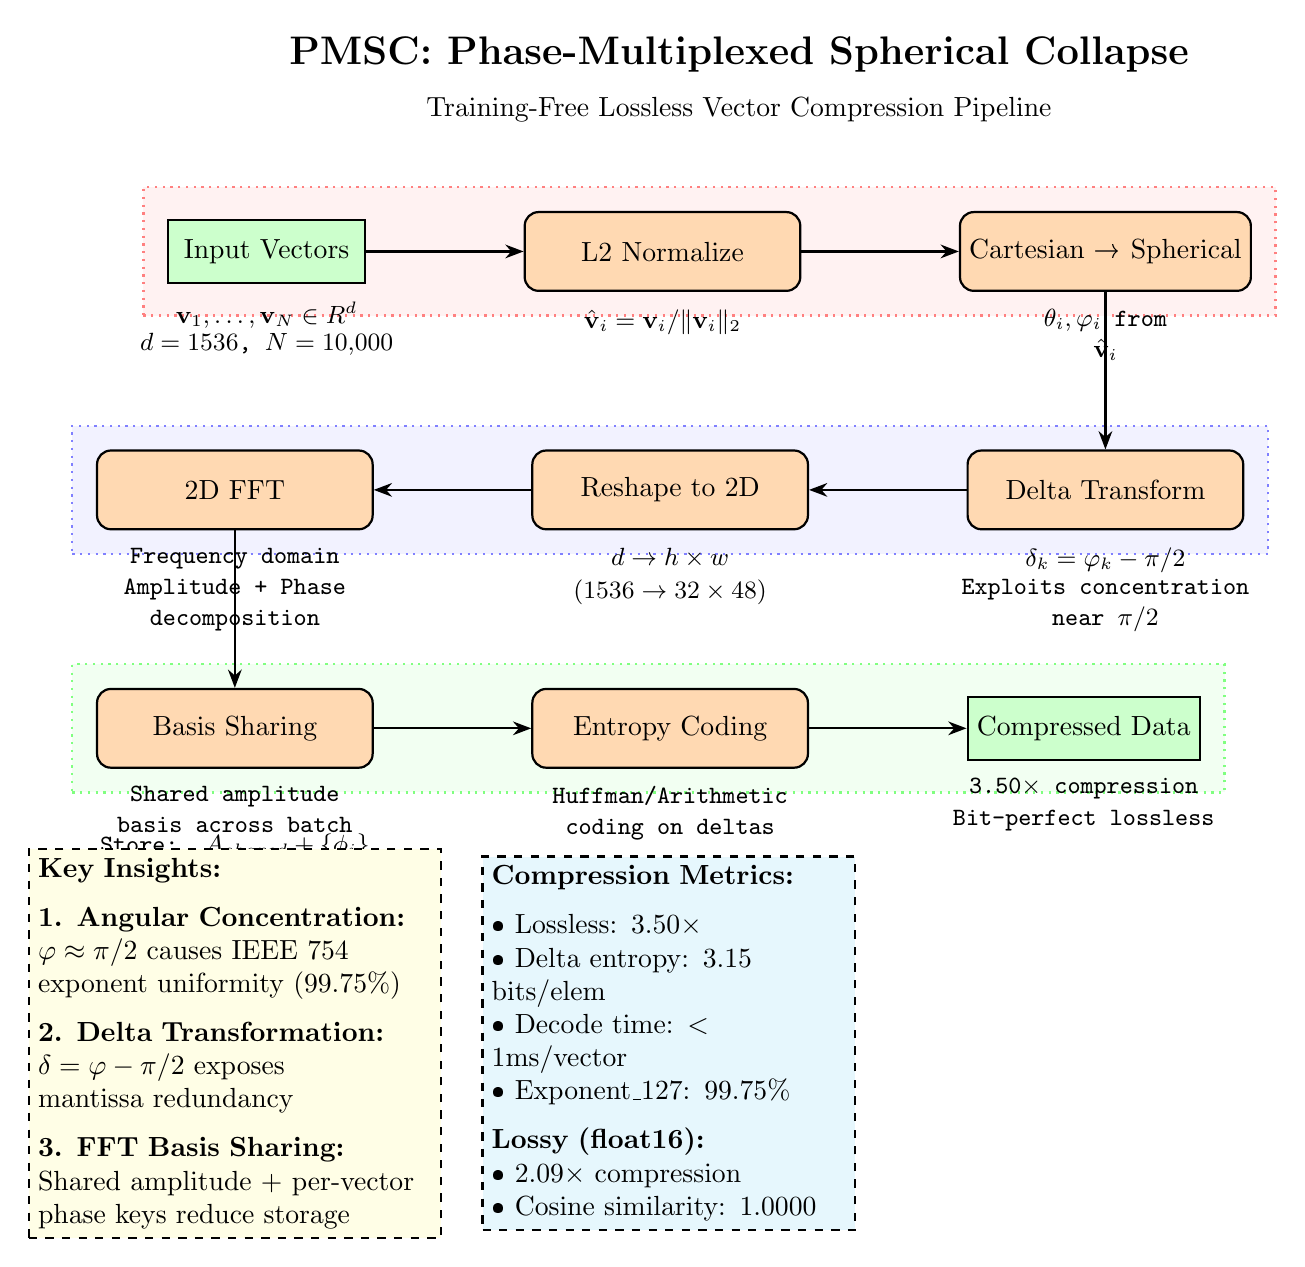
\begin{tikzpicture}[node distance=1.5cm and 2cm]

%% Title
\node[font=\Large\bfseries] at (0, 8) {PMSC: Phase-Multiplexed Spherical Collapse};
\node[font=\normalsize] at (0, 7.3) {Training-Free Lossless Vector Compression Pipeline};

%% ========== STAGE 1: INPUT ==========
\node[databox] (input) at (-6, 5.5) {Input Vectors};
\node[label, below=0.1cm of input] {$\mathbf{v}_1, \dots, \mathbf{v}_N \in \mathbb{R}^d$};
\node[label, below=0.5cm of input] {$d=1536$, $N=10{,}000$};

%% ========== STAGE 2: NORMALIZATION ==========
\node[process, right=of input] (norm) {L2 Normalize};
\node[label, below=0.1cm of norm] {$\hat{\mathbf{v}}_i = \mathbf{v}_i / \|\mathbf{v}_i\|_2$};

%% ========== STAGE 3: SPHERICAL COORDINATES ==========
\node[process, right=of norm] (spherical) {Cartesian → Spherical};
\node[label, below=0.1cm of spherical, align=center] {$\theta_i, \varphi_i$ from\\$\hat{\mathbf{v}}_i$};

%% ========== STAGE 4: DELTA TRANSFORMATION ==========
\node[process, below=2cm of spherical] (delta) {Delta Transform};
\node[label, below=0.1cm of delta] {$\delta_k = \varphi_k - \pi/2$};
\node[label, below=0.5cm of delta, align=center] {Exploits concentration\\near $\pi/2$};

%% ========== STAGE 5: 2D RESHAPE ==========
\node[process, left=of delta] (reshape) {Reshape to 2D};
\node[label, below=0.1cm of reshape] {$d \to h \times w$};
\node[label, below=0.5cm of reshape] {$(1536 \to 32 \times 48)$};

%% ========== STAGE 6: FFT ==========
\node[process, left=of reshape] (fft) {2D FFT};
\node[label, below=0.1cm of fft] {Frequency domain};
\node[label, below=0.5cm of fft, align=center] {Amplitude + Phase\\decomposition};

%% ========== STAGE 7: BASIS SHARING ==========
\node[process, below=2cm of fft] (basis) {Basis Sharing};
\node[label, below=0.1cm of basis, align=center] {Shared amplitude\\basis across batch};
\node[label, below=0.7cm of basis] {Store: $A_{\text{shared}} + \{\phi_i\}$};

%% ========== STAGE 8: COMPRESSION ==========
\node[process, right=of basis] (compress) {Entropy Coding};
\node[label, below=0.1cm of compress, align=center] {Huffman/Arithmetic\\coding on deltas};

%% ========== STAGE 9: OUTPUT ==========
\node[databox, right=of compress] (output) {Compressed Data};
\node[label, below=0.1cm of output] {3.50$\times$ compression};
\node[label, below=0.5cm of output] {Bit-perfect lossless};

%% ========== KEY INSIGHTS BOX ==========
\node[draw, thick, dashed, fill=yellow!10, align=left, text width=5cm, below=1cm of basis] (insights) {
  \textbf{Key Insights:}\\[0.2cm]
  \textbf{1. Angular Concentration:}\\$\varphi \approx \pi/2$ causes IEEE 754\\exponent uniformity (99.75\%)\\[0.2cm]
  \textbf{2. Delta Transformation:}\\$\delta = \varphi - \pi/2$ exposes\\mantissa redundancy\\[0.2cm]
  \textbf{3. FFT Basis Sharing:}\\Shared amplitude + per-vector\\phase keys reduce storage
};

%% ========== METRICS BOX ==========
\node[draw, thick, dashed, fill=cyan!10, align=left, text width=4.5cm, right=0.5cm of insights] (metrics) {
  \textbf{Compression Metrics:}\\[0.2cm]
  • Lossless: 3.50$\times$\\• Delta entropy: 3.15 bits/elem\\• Decode time: $<1$ms/vector\\• Exponent\_127: 99.75\%\\[0.2cm]
  \textbf{Lossy (float16):}\\• 2.09$\times$ compression\\• Cosine similarity: 1.0000
};

%% ========== ARROWS ==========
\draw[arrow] (input) -- (norm);
\draw[arrow] (norm) -- (spherical);
\draw[arrow] (spherical) -- (delta);
\draw[arrow] (delta) -- (reshape);
\draw[arrow] (reshape) -- (fft);
\draw[arrow] (fft) -- (basis);
\draw[arrow] (basis) -- (compress);
\draw[arrow] (compress) -- (output);

%% ========== BACKGROUND GROUPING ==========
\begin{scope}[on background layer]
  \node[draw=red!50, thick, dotted, fill=red!5, fit=(input)(norm)(spherical), inner sep=0.3cm, label={[fill=red!10, font=\small\bfseries]above:Preprocessing}] {};
  \node[draw=blue!50, thick, dotted, fill=blue!5, fit=(delta)(reshape)(fft), inner sep=0.3cm, label={[fill=blue!10, font=\small\bfseries]above:Transform}] {};
  \node[draw=green!50, thick, dotted, fill=green!5, fit=(basis)(compress)(output), inner sep=0.3cm, label={[fill=green!10, font=\small\bfseries]above:Compression}] {};
\end{scope}

\end{tikzpicture}
\end{document}

%% ========== COMPILATION INSTRUCTIONS ==========
%% To compile this diagram:
%% 1. Save as PMSC_ARCHITECTURE_DIAGRAM.tex
%% 2. Run: pdflatex PMSC_ARCHITECTURE_DIAGRAM.tex
%% 3. Output: PMSC_ARCHITECTURE_DIAGRAM.pdf
%%
%% To include in main.tex:
%% \begin{figure}[t]
%%   \centering
%%   %% PMSC Architecture Diagram - TikZ/LaTeX Implementation
%% Author: Ege Berk Türk
%% Date: May 23, 2026
%% Usage: Compile with pdflatex or include in main.tex

\documentclass[border=10pt]{standalone}
\usepackage{tikz}
\usetikzlibrary{shapes.geometric, arrows.meta, positioning, fit, backgrounds, calc}

\tikzset{
  box/.style={rectangle, draw, fill=blue!20, thick, minimum height=1cm, minimum width=3cm, text centered},
  databox/.style={rectangle, draw, fill=green!20, thick, minimum height=0.8cm, minimum width=2.5cm, text centered},
  process/.style={rectangle, draw, fill=orange!30, thick, minimum height=1cm, minimum width=3.5cm, text centered, rounded corners=5pt},
  arrow/.style={-Stealth, thick},
  label/.style={font=\small\ttfamily},
}

\begin{document}
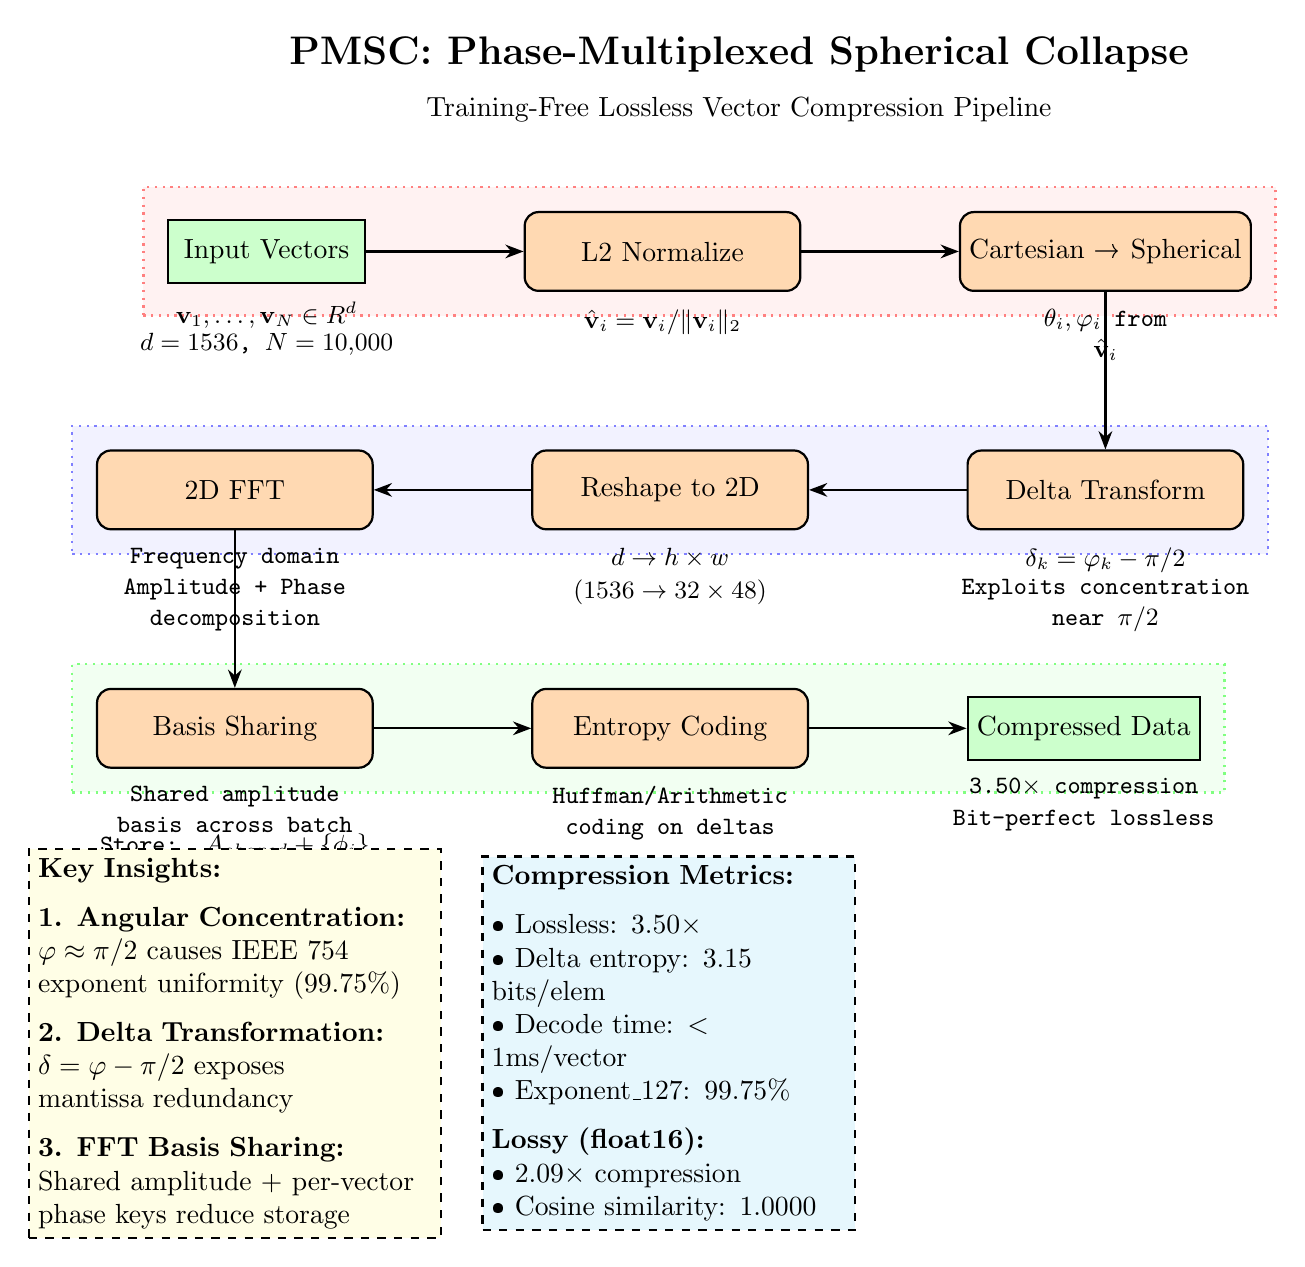
\begin{tikzpicture}[node distance=1.5cm and 2cm]

%% Title
\node[font=\Large\bfseries] at (0, 8) {PMSC: Phase-Multiplexed Spherical Collapse};
\node[font=\normalsize] at (0, 7.3) {Training-Free Lossless Vector Compression Pipeline};

%% ========== STAGE 1: INPUT ==========
\node[databox] (input) at (-6, 5.5) {Input Vectors};
\node[label, below=0.1cm of input] {$\mathbf{v}_1, \dots, \mathbf{v}_N \in \mathbb{R}^d$};
\node[label, below=0.5cm of input] {$d=1536$, $N=10{,}000$};

%% ========== STAGE 2: NORMALIZATION ==========
\node[process, right=of input] (norm) {L2 Normalize};
\node[label, below=0.1cm of norm] {$\hat{\mathbf{v}}_i = \mathbf{v}_i / \|\mathbf{v}_i\|_2$};

%% ========== STAGE 3: SPHERICAL COORDINATES ==========
\node[process, right=of norm] (spherical) {Cartesian → Spherical};
\node[label, below=0.1cm of spherical, align=center] {$\theta_i, \varphi_i$ from\\$\hat{\mathbf{v}}_i$};

%% ========== STAGE 4: DELTA TRANSFORMATION ==========
\node[process, below=2cm of spherical] (delta) {Delta Transform};
\node[label, below=0.1cm of delta] {$\delta_k = \varphi_k - \pi/2$};
\node[label, below=0.5cm of delta, align=center] {Exploits concentration\\near $\pi/2$};

%% ========== STAGE 5: 2D RESHAPE ==========
\node[process, left=of delta] (reshape) {Reshape to 2D};
\node[label, below=0.1cm of reshape] {$d \to h \times w$};
\node[label, below=0.5cm of reshape] {$(1536 \to 32 \times 48)$};

%% ========== STAGE 6: FFT ==========
\node[process, left=of reshape] (fft) {2D FFT};
\node[label, below=0.1cm of fft] {Frequency domain};
\node[label, below=0.5cm of fft, align=center] {Amplitude + Phase\\decomposition};

%% ========== STAGE 7: BASIS SHARING ==========
\node[process, below=2cm of fft] (basis) {Basis Sharing};
\node[label, below=0.1cm of basis, align=center] {Shared amplitude\\basis across batch};
\node[label, below=0.7cm of basis] {Store: $A_{\text{shared}} + \{\phi_i\}$};

%% ========== STAGE 8: COMPRESSION ==========
\node[process, right=of basis] (compress) {Entropy Coding};
\node[label, below=0.1cm of compress, align=center] {Huffman/Arithmetic\\coding on deltas};

%% ========== STAGE 9: OUTPUT ==========
\node[databox, right=of compress] (output) {Compressed Data};
\node[label, below=0.1cm of output] {3.50$\times$ compression};
\node[label, below=0.5cm of output] {Bit-perfect lossless};

%% ========== KEY INSIGHTS BOX ==========
\node[draw, thick, dashed, fill=yellow!10, align=left, text width=5cm, below=1cm of basis] (insights) {
  \textbf{Key Insights:}\\[0.2cm]
  \textbf{1. Angular Concentration:}\\$\varphi \approx \pi/2$ causes IEEE 754\\exponent uniformity (99.75\%)\\[0.2cm]
  \textbf{2. Delta Transformation:}\\$\delta = \varphi - \pi/2$ exposes\\mantissa redundancy\\[0.2cm]
  \textbf{3. FFT Basis Sharing:}\\Shared amplitude + per-vector\\phase keys reduce storage
};

%% ========== METRICS BOX ==========
\node[draw, thick, dashed, fill=cyan!10, align=left, text width=4.5cm, right=0.5cm of insights] (metrics) {
  \textbf{Compression Metrics:}\\[0.2cm]
  • Lossless: 3.50$\times$\\• Delta entropy: 3.15 bits/elem\\• Decode time: $<1$ms/vector\\• Exponent\_127: 99.75\%\\[0.2cm]
  \textbf{Lossy (float16):}\\• 2.09$\times$ compression\\• Cosine similarity: 1.0000
};

%% ========== ARROWS ==========
\draw[arrow] (input) -- (norm);
\draw[arrow] (norm) -- (spherical);
\draw[arrow] (spherical) -- (delta);
\draw[arrow] (delta) -- (reshape);
\draw[arrow] (reshape) -- (fft);
\draw[arrow] (fft) -- (basis);
\draw[arrow] (basis) -- (compress);
\draw[arrow] (compress) -- (output);

%% ========== BACKGROUND GROUPING ==========
\begin{scope}[on background layer]
  \node[draw=red!50, thick, dotted, fill=red!5, fit=(input)(norm)(spherical), inner sep=0.3cm, label={[fill=red!10, font=\small\bfseries]above:Preprocessing}] {};
  \node[draw=blue!50, thick, dotted, fill=blue!5, fit=(delta)(reshape)(fft), inner sep=0.3cm, label={[fill=blue!10, font=\small\bfseries]above:Transform}] {};
  \node[draw=green!50, thick, dotted, fill=green!5, fit=(basis)(compress)(output), inner sep=0.3cm, label={[fill=green!10, font=\small\bfseries]above:Compression}] {};
\end{scope}

\end{tikzpicture}
\end{document}

%% ========== COMPILATION INSTRUCTIONS ==========
%% To compile this diagram:
%% 1. Save as PMSC_ARCHITECTURE_DIAGRAM.tex
%% 2. Run: pdflatex PMSC_ARCHITECTURE_DIAGRAM.tex
%% 3. Output: PMSC_ARCHITECTURE_DIAGRAM.pdf
%%
%% To include in main.tex:
%% \begin{figure}[t]
%%   \centering
%%   %% PMSC Architecture Diagram - TikZ/LaTeX Implementation
%% Author: Ege Berk Türk
%% Date: May 23, 2026
%% Usage: Compile with pdflatex or include in main.tex

\documentclass[border=10pt]{standalone}
\usepackage{tikz}
\usetikzlibrary{shapes.geometric, arrows.meta, positioning, fit, backgrounds, calc}

\tikzset{
  box/.style={rectangle, draw, fill=blue!20, thick, minimum height=1cm, minimum width=3cm, text centered},
  databox/.style={rectangle, draw, fill=green!20, thick, minimum height=0.8cm, minimum width=2.5cm, text centered},
  process/.style={rectangle, draw, fill=orange!30, thick, minimum height=1cm, minimum width=3.5cm, text centered, rounded corners=5pt},
  arrow/.style={-Stealth, thick},
  label/.style={font=\small\ttfamily},
}

\begin{document}
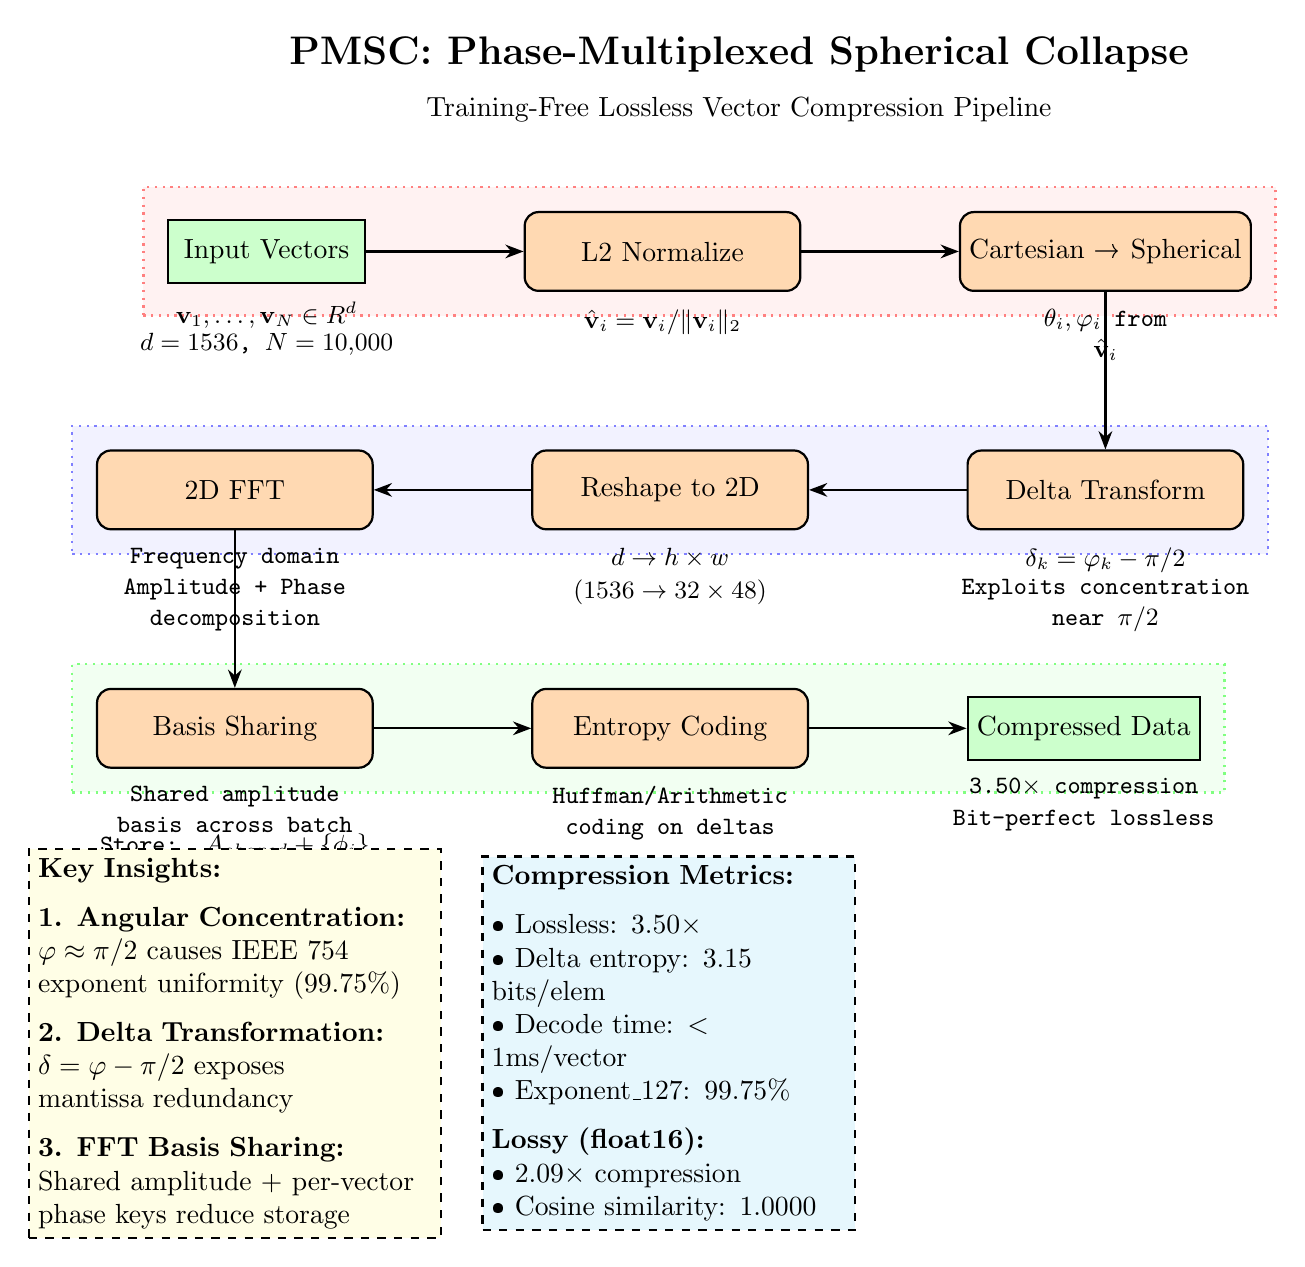
\begin{tikzpicture}[node distance=1.5cm and 2cm]

%% Title
\node[font=\Large\bfseries] at (0, 8) {PMSC: Phase-Multiplexed Spherical Collapse};
\node[font=\normalsize] at (0, 7.3) {Training-Free Lossless Vector Compression Pipeline};

%% ========== STAGE 1: INPUT ==========
\node[databox] (input) at (-6, 5.5) {Input Vectors};
\node[label, below=0.1cm of input] {$\mathbf{v}_1, \dots, \mathbf{v}_N \in \mathbb{R}^d$};
\node[label, below=0.5cm of input] {$d=1536$, $N=10{,}000$};

%% ========== STAGE 2: NORMALIZATION ==========
\node[process, right=of input] (norm) {L2 Normalize};
\node[label, below=0.1cm of norm] {$\hat{\mathbf{v}}_i = \mathbf{v}_i / \|\mathbf{v}_i\|_2$};

%% ========== STAGE 3: SPHERICAL COORDINATES ==========
\node[process, right=of norm] (spherical) {Cartesian → Spherical};
\node[label, below=0.1cm of spherical, align=center] {$\theta_i, \varphi_i$ from\\$\hat{\mathbf{v}}_i$};

%% ========== STAGE 4: DELTA TRANSFORMATION ==========
\node[process, below=2cm of spherical] (delta) {Delta Transform};
\node[label, below=0.1cm of delta] {$\delta_k = \varphi_k - \pi/2$};
\node[label, below=0.5cm of delta, align=center] {Exploits concentration\\near $\pi/2$};

%% ========== STAGE 5: 2D RESHAPE ==========
\node[process, left=of delta] (reshape) {Reshape to 2D};
\node[label, below=0.1cm of reshape] {$d \to h \times w$};
\node[label, below=0.5cm of reshape] {$(1536 \to 32 \times 48)$};

%% ========== STAGE 6: FFT ==========
\node[process, left=of reshape] (fft) {2D FFT};
\node[label, below=0.1cm of fft] {Frequency domain};
\node[label, below=0.5cm of fft, align=center] {Amplitude + Phase\\decomposition};

%% ========== STAGE 7: BASIS SHARING ==========
\node[process, below=2cm of fft] (basis) {Basis Sharing};
\node[label, below=0.1cm of basis, align=center] {Shared amplitude\\basis across batch};
\node[label, below=0.7cm of basis] {Store: $A_{\text{shared}} + \{\phi_i\}$};

%% ========== STAGE 8: COMPRESSION ==========
\node[process, right=of basis] (compress) {Entropy Coding};
\node[label, below=0.1cm of compress, align=center] {Huffman/Arithmetic\\coding on deltas};

%% ========== STAGE 9: OUTPUT ==========
\node[databox, right=of compress] (output) {Compressed Data};
\node[label, below=0.1cm of output] {3.50$\times$ compression};
\node[label, below=0.5cm of output] {Bit-perfect lossless};

%% ========== KEY INSIGHTS BOX ==========
\node[draw, thick, dashed, fill=yellow!10, align=left, text width=5cm, below=1cm of basis] (insights) {
  \textbf{Key Insights:}\\[0.2cm]
  \textbf{1. Angular Concentration:}\\$\varphi \approx \pi/2$ causes IEEE 754\\exponent uniformity (99.75\%)\\[0.2cm]
  \textbf{2. Delta Transformation:}\\$\delta = \varphi - \pi/2$ exposes\\mantissa redundancy\\[0.2cm]
  \textbf{3. FFT Basis Sharing:}\\Shared amplitude + per-vector\\phase keys reduce storage
};

%% ========== METRICS BOX ==========
\node[draw, thick, dashed, fill=cyan!10, align=left, text width=4.5cm, right=0.5cm of insights] (metrics) {
  \textbf{Compression Metrics:}\\[0.2cm]
  • Lossless: 3.50$\times$\\• Delta entropy: 3.15 bits/elem\\• Decode time: $<1$ms/vector\\• Exponent\_127: 99.75\%\\[0.2cm]
  \textbf{Lossy (float16):}\\• 2.09$\times$ compression\\• Cosine similarity: 1.0000
};

%% ========== ARROWS ==========
\draw[arrow] (input) -- (norm);
\draw[arrow] (norm) -- (spherical);
\draw[arrow] (spherical) -- (delta);
\draw[arrow] (delta) -- (reshape);
\draw[arrow] (reshape) -- (fft);
\draw[arrow] (fft) -- (basis);
\draw[arrow] (basis) -- (compress);
\draw[arrow] (compress) -- (output);

%% ========== BACKGROUND GROUPING ==========
\begin{scope}[on background layer]
  \node[draw=red!50, thick, dotted, fill=red!5, fit=(input)(norm)(spherical), inner sep=0.3cm, label={[fill=red!10, font=\small\bfseries]above:Preprocessing}] {};
  \node[draw=blue!50, thick, dotted, fill=blue!5, fit=(delta)(reshape)(fft), inner sep=0.3cm, label={[fill=blue!10, font=\small\bfseries]above:Transform}] {};
  \node[draw=green!50, thick, dotted, fill=green!5, fit=(basis)(compress)(output), inner sep=0.3cm, label={[fill=green!10, font=\small\bfseries]above:Compression}] {};
\end{scope}

\end{tikzpicture}
\end{document}

%% ========== COMPILATION INSTRUCTIONS ==========
%% To compile this diagram:
%% 1. Save as PMSC_ARCHITECTURE_DIAGRAM.tex
%% 2. Run: pdflatex PMSC_ARCHITECTURE_DIAGRAM.tex
%% 3. Output: PMSC_ARCHITECTURE_DIAGRAM.pdf
%%
%% To include in main.tex:
%% \begin{figure}[t]
%%   \centering
%%   %% PMSC Architecture Diagram - TikZ/LaTeX Implementation
%% Author: Ege Berk Türk
%% Date: May 23, 2026
%% Usage: Compile with pdflatex or include in main.tex

\documentclass[border=10pt]{standalone}
\usepackage{tikz}
\usetikzlibrary{shapes.geometric, arrows.meta, positioning, fit, backgrounds, calc}

\tikzset{
  box/.style={rectangle, draw, fill=blue!20, thick, minimum height=1cm, minimum width=3cm, text centered},
  databox/.style={rectangle, draw, fill=green!20, thick, minimum height=0.8cm, minimum width=2.5cm, text centered},
  process/.style={rectangle, draw, fill=orange!30, thick, minimum height=1cm, minimum width=3.5cm, text centered, rounded corners=5pt},
  arrow/.style={-Stealth, thick},
  label/.style={font=\small\ttfamily},
}

\begin{document}
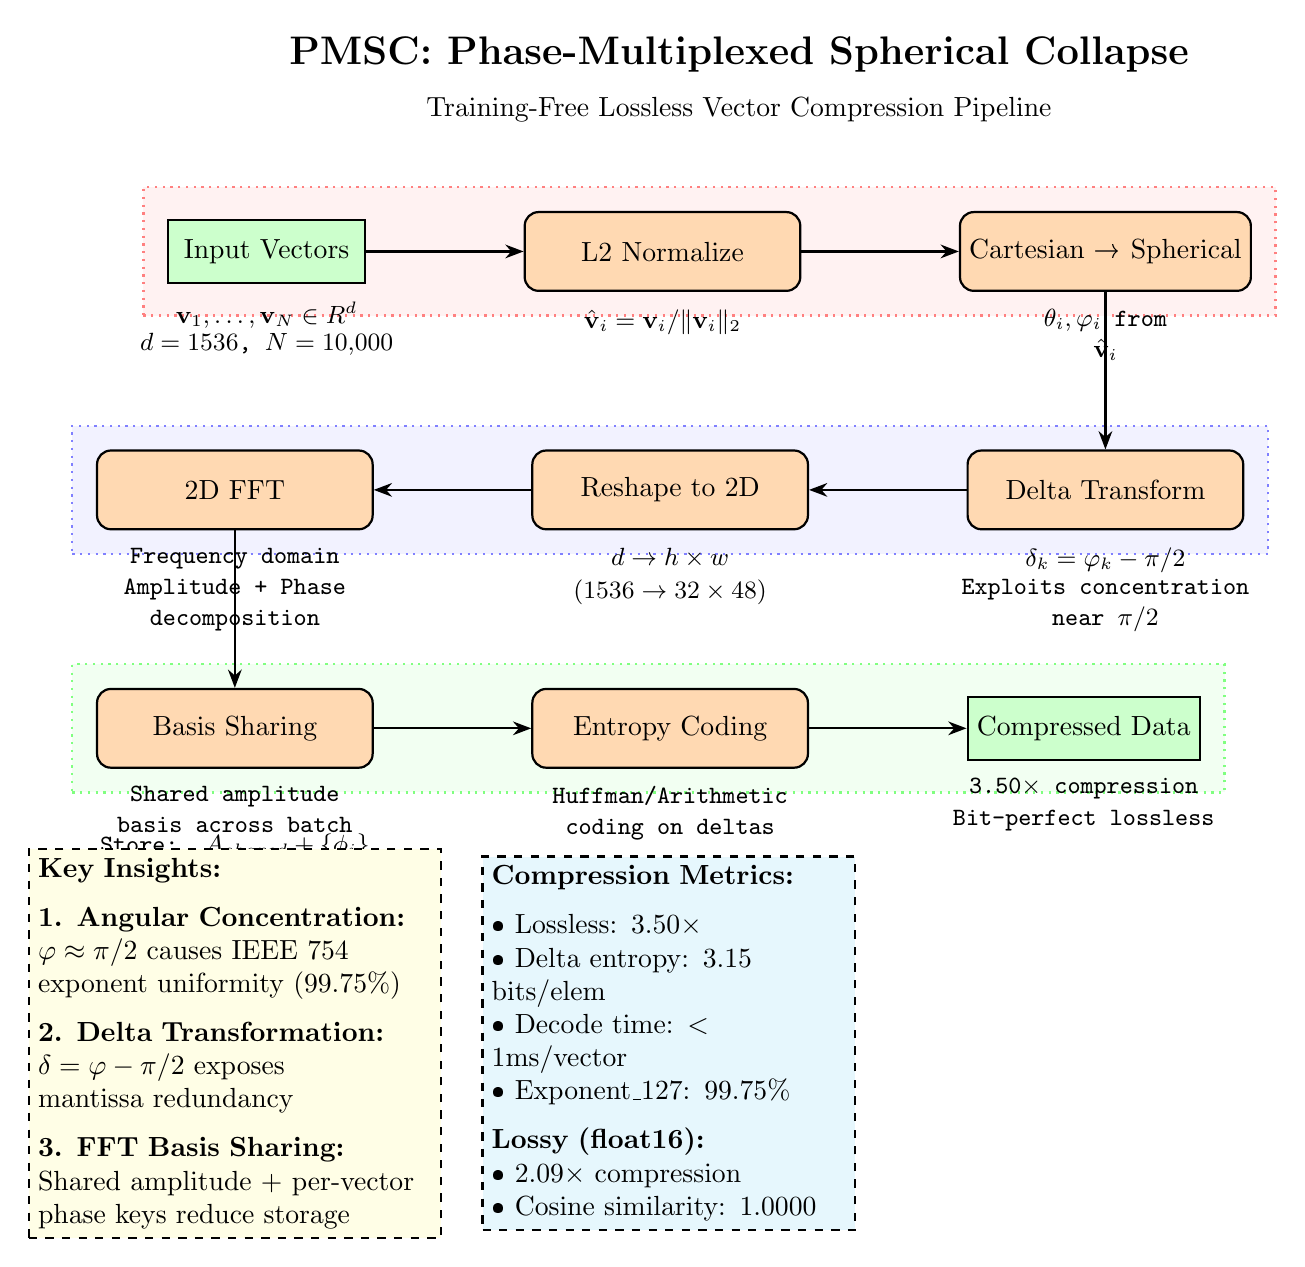
\begin{tikzpicture}[node distance=1.5cm and 2cm]

%% Title
\node[font=\Large\bfseries] at (0, 8) {PMSC: Phase-Multiplexed Spherical Collapse};
\node[font=\normalsize] at (0, 7.3) {Training-Free Lossless Vector Compression Pipeline};

%% ========== STAGE 1: INPUT ==========
\node[databox] (input) at (-6, 5.5) {Input Vectors};
\node[label, below=0.1cm of input] {$\mathbf{v}_1, \dots, \mathbf{v}_N \in \mathbb{R}^d$};
\node[label, below=0.5cm of input] {$d=1536$, $N=10{,}000$};

%% ========== STAGE 2: NORMALIZATION ==========
\node[process, right=of input] (norm) {L2 Normalize};
\node[label, below=0.1cm of norm] {$\hat{\mathbf{v}}_i = \mathbf{v}_i / \|\mathbf{v}_i\|_2$};

%% ========== STAGE 3: SPHERICAL COORDINATES ==========
\node[process, right=of norm] (spherical) {Cartesian → Spherical};
\node[label, below=0.1cm of spherical, align=center] {$\theta_i, \varphi_i$ from\\$\hat{\mathbf{v}}_i$};

%% ========== STAGE 4: DELTA TRANSFORMATION ==========
\node[process, below=2cm of spherical] (delta) {Delta Transform};
\node[label, below=0.1cm of delta] {$\delta_k = \varphi_k - \pi/2$};
\node[label, below=0.5cm of delta, align=center] {Exploits concentration\\near $\pi/2$};

%% ========== STAGE 5: 2D RESHAPE ==========
\node[process, left=of delta] (reshape) {Reshape to 2D};
\node[label, below=0.1cm of reshape] {$d \to h \times w$};
\node[label, below=0.5cm of reshape] {$(1536 \to 32 \times 48)$};

%% ========== STAGE 6: FFT ==========
\node[process, left=of reshape] (fft) {2D FFT};
\node[label, below=0.1cm of fft] {Frequency domain};
\node[label, below=0.5cm of fft, align=center] {Amplitude + Phase\\decomposition};

%% ========== STAGE 7: BASIS SHARING ==========
\node[process, below=2cm of fft] (basis) {Basis Sharing};
\node[label, below=0.1cm of basis, align=center] {Shared amplitude\\basis across batch};
\node[label, below=0.7cm of basis] {Store: $A_{\text{shared}} + \{\phi_i\}$};

%% ========== STAGE 8: COMPRESSION ==========
\node[process, right=of basis] (compress) {Entropy Coding};
\node[label, below=0.1cm of compress, align=center] {Huffman/Arithmetic\\coding on deltas};

%% ========== STAGE 9: OUTPUT ==========
\node[databox, right=of compress] (output) {Compressed Data};
\node[label, below=0.1cm of output] {3.50$\times$ compression};
\node[label, below=0.5cm of output] {Bit-perfect lossless};

%% ========== KEY INSIGHTS BOX ==========
\node[draw, thick, dashed, fill=yellow!10, align=left, text width=5cm, below=1cm of basis] (insights) {
  \textbf{Key Insights:}\\[0.2cm]
  \textbf{1. Angular Concentration:}\\$\varphi \approx \pi/2$ causes IEEE 754\\exponent uniformity (99.75\%)\\[0.2cm]
  \textbf{2. Delta Transformation:}\\$\delta = \varphi - \pi/2$ exposes\\mantissa redundancy\\[0.2cm]
  \textbf{3. FFT Basis Sharing:}\\Shared amplitude + per-vector\\phase keys reduce storage
};

%% ========== METRICS BOX ==========
\node[draw, thick, dashed, fill=cyan!10, align=left, text width=4.5cm, right=0.5cm of insights] (metrics) {
  \textbf{Compression Metrics:}\\[0.2cm]
  • Lossless: 3.50$\times$\\• Delta entropy: 3.15 bits/elem\\• Decode time: $<1$ms/vector\\• Exponent\_127: 99.75\%\\[0.2cm]
  \textbf{Lossy (float16):}\\• 2.09$\times$ compression\\• Cosine similarity: 1.0000
};

%% ========== ARROWS ==========
\draw[arrow] (input) -- (norm);
\draw[arrow] (norm) -- (spherical);
\draw[arrow] (spherical) -- (delta);
\draw[arrow] (delta) -- (reshape);
\draw[arrow] (reshape) -- (fft);
\draw[arrow] (fft) -- (basis);
\draw[arrow] (basis) -- (compress);
\draw[arrow] (compress) -- (output);

%% ========== BACKGROUND GROUPING ==========
\begin{scope}[on background layer]
  \node[draw=red!50, thick, dotted, fill=red!5, fit=(input)(norm)(spherical), inner sep=0.3cm, label={[fill=red!10, font=\small\bfseries]above:Preprocessing}] {};
  \node[draw=blue!50, thick, dotted, fill=blue!5, fit=(delta)(reshape)(fft), inner sep=0.3cm, label={[fill=blue!10, font=\small\bfseries]above:Transform}] {};
  \node[draw=green!50, thick, dotted, fill=green!5, fit=(basis)(compress)(output), inner sep=0.3cm, label={[fill=green!10, font=\small\bfseries]above:Compression}] {};
\end{scope}

\end{tikzpicture}
\end{document}

%% ========== COMPILATION INSTRUCTIONS ==========
%% To compile this diagram:
%% 1. Save as PMSC_ARCHITECTURE_DIAGRAM.tex
%% 2. Run: pdflatex PMSC_ARCHITECTURE_DIAGRAM.tex
%% 3. Output: PMSC_ARCHITECTURE_DIAGRAM.pdf
%%
%% To include in main.tex:
%% \begin{figure}[t]
%%   \centering
%%   \input{PMSC_ARCHITECTURE_DIAGRAM.tex}
%%   \caption{PMSC Architecture: The complete pipeline from input vectors
%%            to compressed output, showing the three key stages: 
%%            Preprocessing (normalization, spherical coordinates),
%%            Transform (delta transformation, 2D FFT), and
%%            Compression (basis sharing, entropy coding).}
%%   \label{fig:pmsc_architecture}
%% \end{figure}
%%
%% Or include as compiled PDF:
%% \begin{figure}[t]
%%   \centering
%%   \includegraphics[width=\textwidth]{PMSC_ARCHITECTURE_DIAGRAM.pdf}
%%   \caption{PMSC Architecture Pipeline}
%%   \label{fig:pmsc_architecture}
%% \end{figure}

%%   \caption{PMSC Architecture: The complete pipeline from input vectors
%%            to compressed output, showing the three key stages: 
%%            Preprocessing (normalization, spherical coordinates),
%%            Transform (delta transformation, 2D FFT), and
%%            Compression (basis sharing, entropy coding).}
%%   \label{fig:pmsc_architecture}
%% \end{figure}
%%
%% Or include as compiled PDF:
%% \begin{figure}[t]
%%   \centering
%%   \includegraphics[width=\textwidth]{PMSC_ARCHITECTURE_DIAGRAM.pdf}
%%   \caption{PMSC Architecture Pipeline}
%%   \label{fig:pmsc_architecture}
%% \end{figure}

%%   \caption{PMSC Architecture: The complete pipeline from input vectors
%%            to compressed output, showing the three key stages: 
%%            Preprocessing (normalization, spherical coordinates),
%%            Transform (delta transformation, 2D FFT), and
%%            Compression (basis sharing, entropy coding).}
%%   \label{fig:pmsc_architecture}
%% \end{figure}
%%
%% Or include as compiled PDF:
%% \begin{figure}[t]
%%   \centering
%%   \includegraphics[width=\textwidth]{PMSC_ARCHITECTURE_DIAGRAM.pdf}
%%   \caption{PMSC Architecture Pipeline}
%%   \label{fig:pmsc_architecture}
%% \end{figure}

%%   \caption{PMSC Architecture: The complete pipeline from input vectors
%%            to compressed output, showing the three key stages: 
%%            Preprocessing (normalization, spherical coordinates),
%%            Transform (delta transformation, 2D FFT), and
%%            Compression (basis sharing, entropy coding).}
%%   \label{fig:pmsc_architecture}
%% \end{figure}
%%
%% Or include as compiled PDF:
%% \begin{figure}[t]
%%   \centering
%%   \includegraphics[width=\textwidth]{PMSC_ARCHITECTURE_DIAGRAM.pdf}
%%   \caption{PMSC Architecture Pipeline}
%%   \label{fig:pmsc_architecture}
%% \end{figure}
